\section{Blockchain Basics and Bitcoin}
\subsection{Hash Functions}
\paragraph{Properties:}
\begin{itemize}
    \item Arbitrary input size
    \item Fixed-output size
    \item Deterministic (equal inputs hash to the same value)
    \item Uniform (inputs are mapped evenly to the space of possible outputs)
    \item Efficient (should be fast to compute)
\end{itemize}
\textbf{Note:} Collisions always exists since input space is unbounded. However, cryptographic hash functions ensure collisions are hard to find
\paragraph{Cryptographic hash functions properties:}
\begin{itemize}
    \item \textbf{Pre-image resistant: }Given $y \in Y,$ it is infeasible to find $x \in X$ such that $h(x)=y$
    \item \textbf{Second pre-image resistant: }Given $x \in X,$ it is infeasible to find $x^{\prime} \in X$ such that $x \neq x^{\prime}$ and $h(x)=h\left(x^{\prime}\right)$
    \item \textbf{Collision resistance: }It is infeasible to find a pair $\left(x, x^{\prime}\right) \in X \times X$ such that $x \neq x^{\prime}$ and $h(x)=$ $h\left(x^{\prime}\right)$. This implies second-pre-image resistance
\end{itemize}
\paragraph{Applications: }
\begin{itemize}
    \item \textbf{Data equality: } If we know that $h(x)=h(y)$ and $h$ is a cryptographic hash function, then it is safe to assume that $x=y$
    \item \textbf{Data integrity: } 
    \begin{itemize}
        \item To verify the integrity a piece of data $\color{blue}d$, we can remember its hash, $\texttt{\textcolor{blue}{hash}}$ = $\textcolor{blue}{h}(d)$
        \item Later, when we obtain $\color{red}d^{\prime}$ from $\texttt{\textcolor{red}{untrusted source}}$, we can verify whether $\texttt{\textcolor{blue}{hash}}$ = $\color{red}h\left(d^{\prime}\right)$ to check whether $\color{blue}d$ = $\color{red}d^{\prime}$
        \item Useful because \texttt{\textcolor{blue}{hash}} is small (e.g. 256 bits)
    \end{itemize}{}
\end{itemize}{}
\paragraph{Crypto puzzles: }
\begin{itemize}
    \item \textbf{Puzzle-friendly} For any output $\color{blue}y$, if $\color{red}r$ is chosen from a probability distribution with high min-entropy, then it is infeasible to find $\color{green}x$ such that $h(\texttt{\textcolor{red}{r}} | \texttt{\textcolor{green}{x}})=\texttt{\textcolor{blue}{y}}$
    \item \textbf{Search puzzle:} Given a puzzle ID $\color{blue}id,$ chosen from a probability distribution with high min-entropy (min-entropy = minimum amount of randomness in a distribution or how good it is "shuffled"), and an output target $\color{blue}T \subseteq Y$, find a solution $\color{green}x$ such that $h(\texttt{\textcolor{blue}{id}} | \texttt{\textcolor{green}{x}}) \in \texttt{\textcolor{blue}{T}}$. Puzzle-friendliness implies that no solving strategy is much better than trying random values of $\color{green}x$
\end{itemize}{}
\subsection{Merkle Trees}
\begin{minipage}{.5\linewidth}
    \centering      
    \def\svgwidth{\columnwidth}
    %% Creator: Inkscape inkscape 0.92.4, www.inkscape.org
%% PDF/EPS/PS + LaTeX output extension by Johan Engelen, 2010
%% Accompanies image file 'L2_merkle_trees.pdf' (pdf, eps, ps)
%%
%% To include the image in your LaTeX document, write
%%   \input{<filename>.pdf_tex}
%%  instead of
%%   \includegraphics{<filename>.pdf}
%% To scale the image, write
%%   \def\svgwidth{<desired width>}
%%   \input{<filename>.pdf_tex}
%%  instead of
%%   \includegraphics[width=<desired width>]{<filename>.pdf}
%%
%% Images with a different path to the parent latex file can
%% be accessed with the `import' package (which may need to be
%% installed) using
%%   \usepackage{import}
%% in the preamble, and then including the image with
%%   \import{<path to file>}{<filename>.pdf_tex}
%% Alternatively, one can specify
%%   \graphicspath{{<path to file>/}}
%% 
%% For more information, please see info/svg-inkscape on CTAN:
%%   http://tug.ctan.org/tex-archive/info/svg-inkscape
%%
\begingroup%
  \makeatletter%
  \providecommand\color[2][]{%
    \errmessage{(Inkscape) Color is used for the text in Inkscape, but the package 'color.sty' is not loaded}%
    \renewcommand\color[2][]{}%
  }%
  \providecommand\transparent[1]{%
    \errmessage{(Inkscape) Transparency is used (non-zero) for the text in Inkscape, but the package 'transparent.sty' is not loaded}%
    \renewcommand\transparent[1]{}%
  }%
  \providecommand\rotatebox[2]{#2}%
  \newcommand*\fsize{\dimexpr\f@size pt\relax}%
  \newcommand*\lineheight[1]{\fontsize{\fsize}{#1\fsize}\selectfont}%
  \ifx\svgwidth\undefined%
    \setlength{\unitlength}{720bp}%
    \ifx\svgscale\undefined%
      \relax%
    \else%
      \setlength{\unitlength}{\unitlength * \real{\svgscale}}%
    \fi%
  \else%
    \setlength{\unitlength}{\svgwidth}%
  \fi%
  \global\let\svgwidth\undefined%
  \global\let\svgscale\undefined%
  \makeatother%
  \begin{picture}(1,0.75)%
    \lineheight{1}%
    \setlength\tabcolsep{0pt}%
    \put(0,0){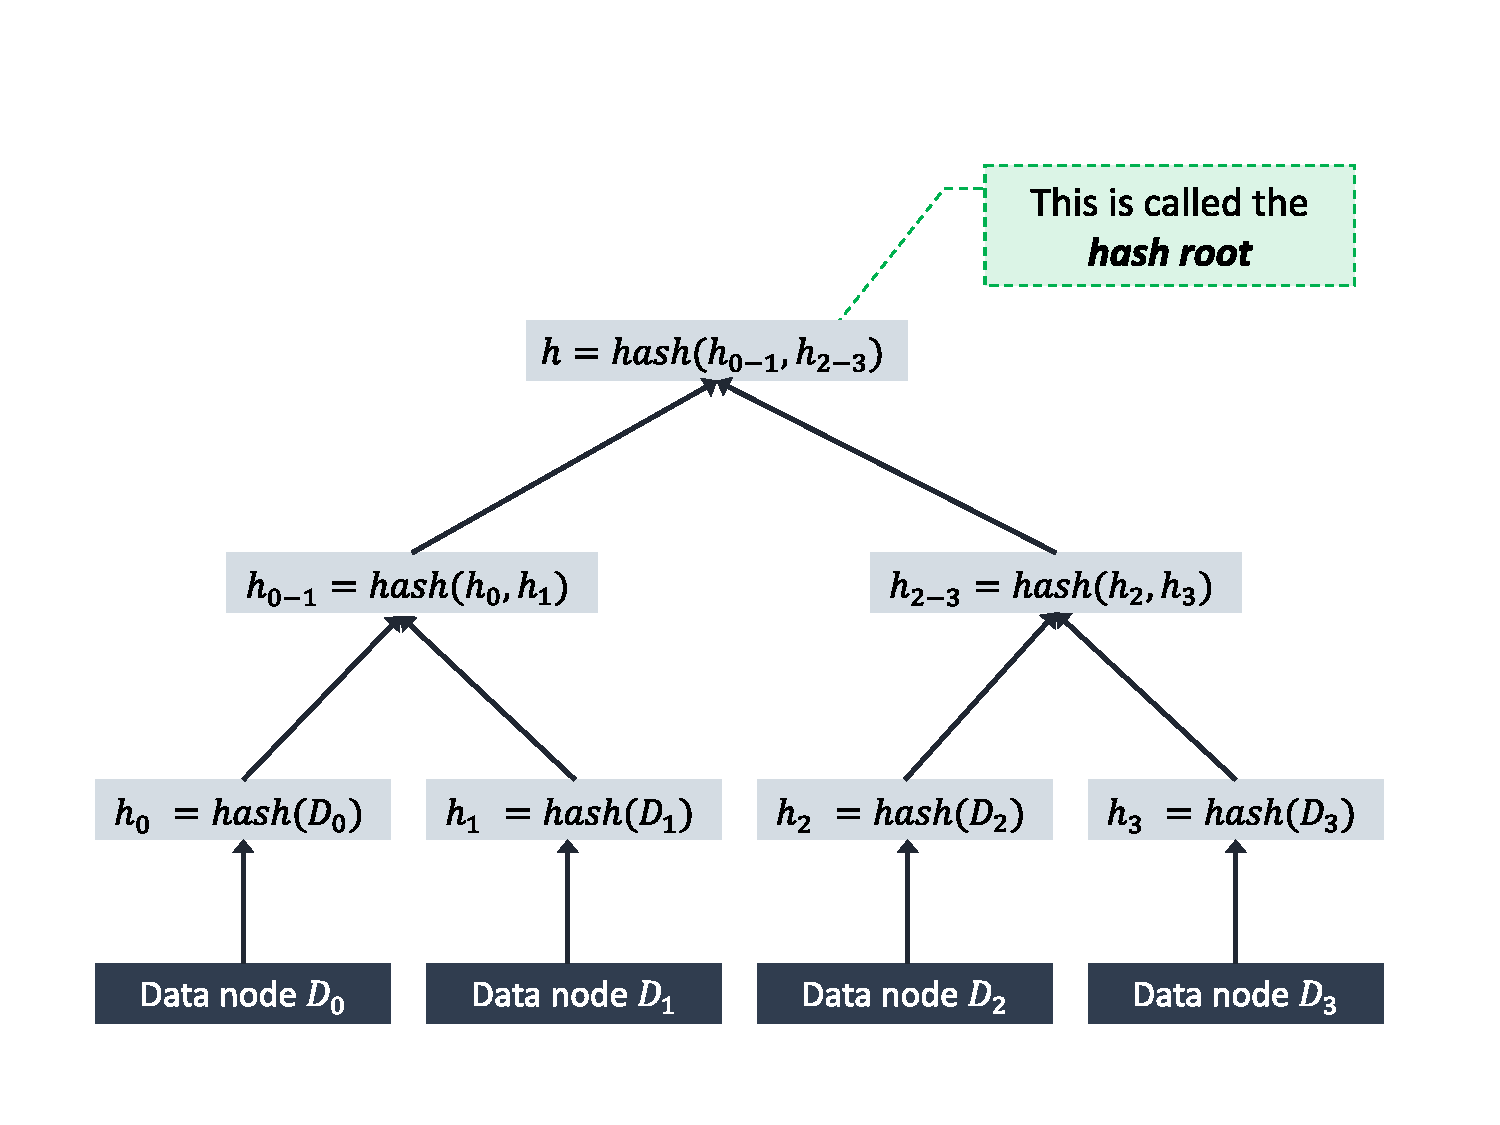
\includegraphics[width=\unitlength,page=1]{Figures/L2_merkle_trees.pdf}}%
  \end{picture}%
\endgroup%
    
\end{minipage}
\begin{minipage}{.5\linewidth}
    \centering      
    \def\svgwidth{\columnwidth}
    %% Creator: Inkscape inkscape 0.92.4, www.inkscape.org
%% PDF/EPS/PS + LaTeX output extension by Johan Engelen, 2010
%% Accompanies image file 'L2_merkle_trees_verification.pdf' (pdf, eps, ps)
%%
%% To include the image in your LaTeX document, write
%%   \input{<filename>.pdf_tex}
%%  instead of
%%   \includegraphics{<filename>.pdf}
%% To scale the image, write
%%   \def\svgwidth{<desired width>}
%%   \input{<filename>.pdf_tex}
%%  instead of
%%   \includegraphics[width=<desired width>]{<filename>.pdf}
%%
%% Images with a different path to the parent latex file can
%% be accessed with the `import' package (which may need to be
%% installed) using
%%   \usepackage{import}
%% in the preamble, and then including the image with
%%   \import{<path to file>}{<filename>.pdf_tex}
%% Alternatively, one can specify
%%   \graphicspath{{<path to file>/}}
%% 
%% For more information, please see info/svg-inkscape on CTAN:
%%   http://tug.ctan.org/tex-archive/info/svg-inkscape
%%
\begingroup%
  \makeatletter%
  \providecommand\color[2][]{%
    \errmessage{(Inkscape) Color is used for the text in Inkscape, but the package 'color.sty' is not loaded}%
    \renewcommand\color[2][]{}%
  }%
  \providecommand\transparent[1]{%
    \errmessage{(Inkscape) Transparency is used (non-zero) for the text in Inkscape, but the package 'transparent.sty' is not loaded}%
    \renewcommand\transparent[1]{}%
  }%
  \providecommand\rotatebox[2]{#2}%
  \newcommand*\fsize{\dimexpr\f@size pt\relax}%
  \newcommand*\lineheight[1]{\fontsize{\fsize}{#1\fsize}\selectfont}%
  \ifx\svgwidth\undefined%
    \setlength{\unitlength}{720bp}%
    \ifx\svgscale\undefined%
      \relax%
    \else%
      \setlength{\unitlength}{\unitlength * \real{\svgscale}}%
    \fi%
  \else%
    \setlength{\unitlength}{\svgwidth}%
  \fi%
  \global\let\svgwidth\undefined%
  \global\let\svgscale\undefined%
  \makeatother%
  \begin{picture}(1,0.75)%
    \lineheight{1}%
    \setlength\tabcolsep{0pt}%
    \put(0,0){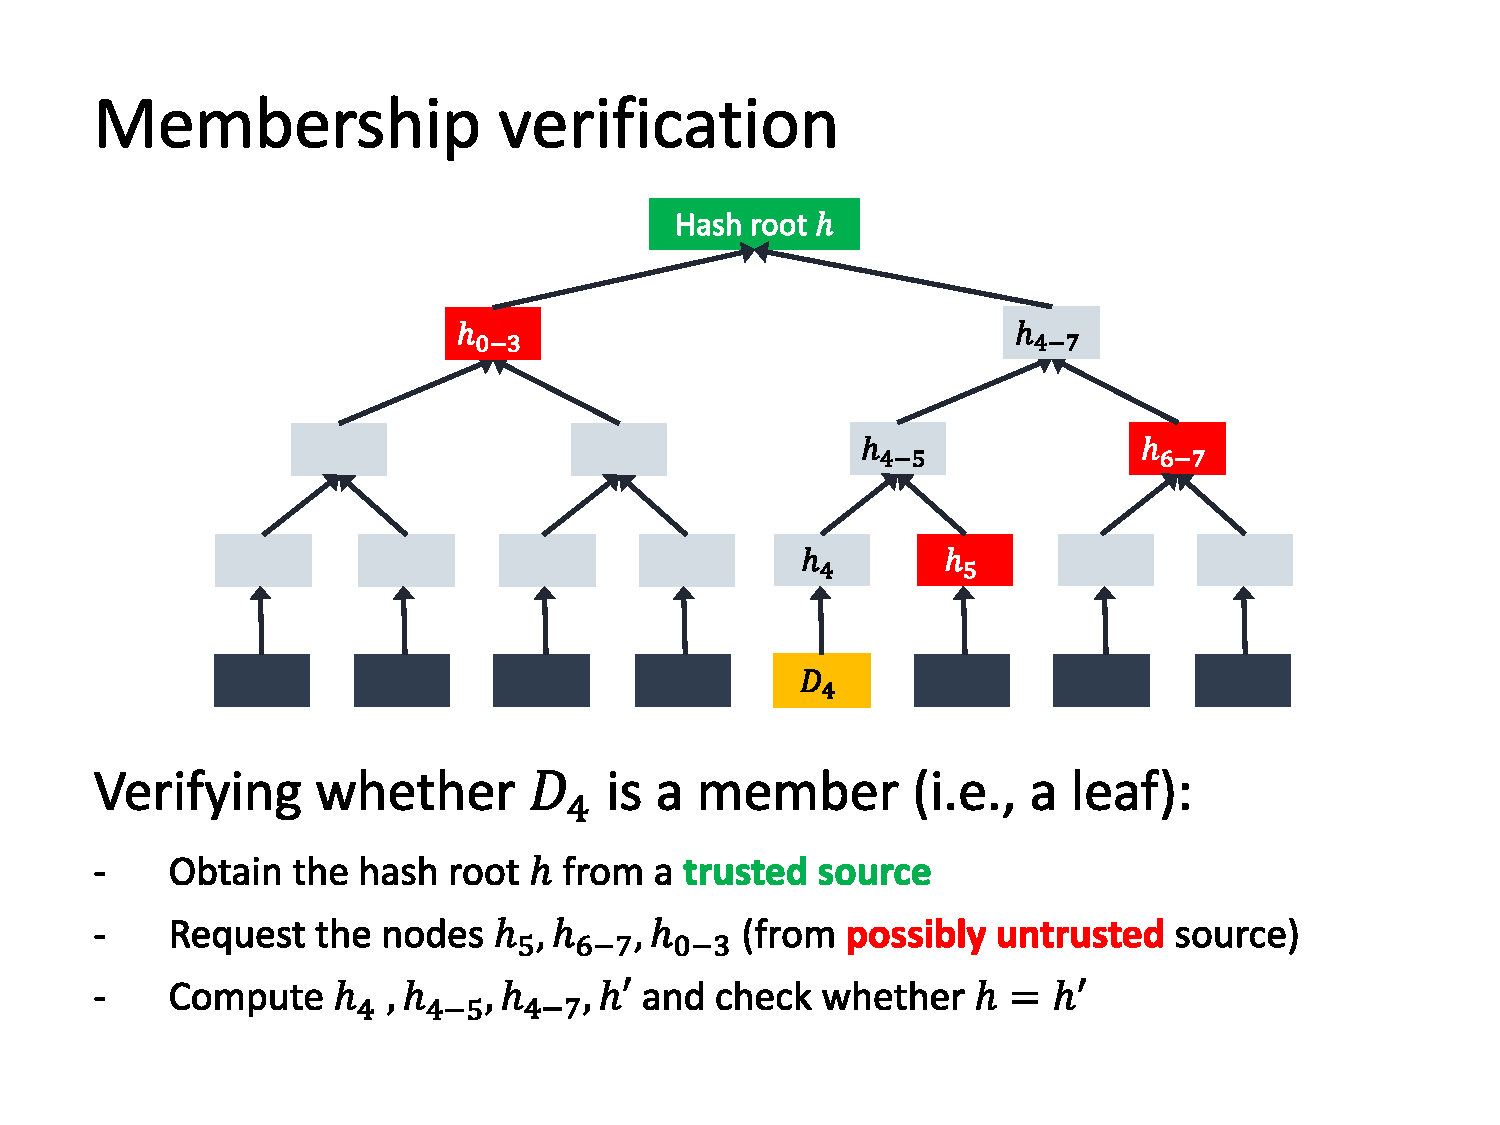
\includegraphics[width=\unitlength,page=1]{Figures/L2_merkle_trees_verification.pdf}}%
  \end{picture}%
\endgroup%
    
\end{minipage}
Membership verification requires $\color{blue}\log (n)$ elements. Useful when the set of data elements is large
\subsection{Digital Signatures}
\textbf{High-level goal: } allow only one user to sign but anyone to verify the signature\newline
\textbf{API for signatures: }
\begin{itemize}
    \item $(\textcolor{red}{sk}, \textcolor{green}{pk})=\texttt{\textcolor{blue}{generateKeys}}(keySize)$
        \begin{itemize}
            \item $\color{red}sk$ is the  $\texttt{\textcolor{red}{secret key}}$, which the owner keeps in private
            \item $\color{green}pk$ is the $\texttt{\textcolor{green}{public key}}$, which is distributed to all users
        \end{itemize}{} 
\item$\textcolor{orange}{sig}$ = $\texttt{\textcolor{blue}{sign}}(\textcolor{red}{sk}, msg)$
\item $\texttt{\textcolor{blue}{verify}}(\textcolor{green}{pk}, msg,\textcolor{orange}{sig})$
\end{itemize}{}
\paragraph{Establish Identity: }
\begin{itemize}
    \item User generates $(\texttt{\textcolor{red}{sk}}, \texttt{\textcolor{green}{pk}})$ key pair
    \item $\texttt{\textcolor{blue}{hash}}(\textcolor{green}{pk})$ is the public name of the user
    \item $\color{red}sk$ allows the user to endorse a statements $stmt$ using a digital signature
    \item $\color{orange}sig$ = $\texttt{\textcolor{blue}{sign}}(\textcolor{red}{sk}, stmt)$
    \item anyone can verify statements endorsed by the user using $\texttt{\textcolor{blue}{verify}}(\textcolor{green}{pk}, \text {stmt}, \textcolor{orange}{sig})$
\end{itemize}
\subsection{Bitcoin Basics}
\paragraph{Distributed Consensus: }
\begin{itemize}
    \item \textbf{Termination: } Every correct process decides on some value
    \item \textbf{Agreement: }  All correct processes decide on the same value
    \item \textbf{Validity: }  If all correct processes propose the same value, then any correct process must decide on that value
\end{itemize}
Traditional motivation: reliability in distributed systems (node replication)
\paragraph{Distributed ledger via consensus: }
\begin{itemize}
    \item To make a transaction, users broadcast transactions to the network nodes
    \item All nodes have a sequence of all blocks of agreed transactions they have reached consensus on
    \item Each node has a set of outstanding transactions (to be added to a block in the blockchain)
\end{itemize}
\textbf{Problems: }
\begin{itemize}
    \item Nodes may crash 
    \item Nodes may be malicious
    \item Network is imperfect
    \begin{itemize}
        \item Not all pair of nodes are connected
        \item Messages may have arbitrary delays
        \item No global time
        \item Nodes may fail 
    \end{itemize}{}
\end{itemize}
\paragraph{Simplified Bitcoin consensus protocol: }
\begin{enumerate}
    \item New transactions are broadcast to all nodes
    \item Each node collects new transactions into a block
    \item In each round, a \texttt{\textcolor{green}{random node}} gets to broadcast its block
    \item Other nodes accept the block only if all transactions in it are valid (unspent, valid signatures)
    \item Nodes express their acceptance of the block by including its hash in the next block they create
\end{enumerate}{}
\textbf{Note: }  \texttt{\textcolor{green}{random node}} selection: 
Select nodes in proportion to a resource that no one can monopolize. Several schemes:
\begin{itemize}
    \item In proportion to computing power: \textcolor{blue}{proof-of-work} used by Bitcoin
    \item In proportion to ownership: \textcolor{blue}{proof-of-stake}
    \item others
\end{itemize}{}
\paragraph{Proof of work:\newline}
\begin{minipage}{0.75\linewidth}
    \def\svgwidth{\columnwidth}
    %% Creator: Inkscape inkscape 0.92.4, www.inkscape.org
%% PDF/EPS/PS + LaTeX output extension by Johan Engelen, 2010
%% Accompanies image file 'L2_PoW.pdf' (pdf, eps, ps)
%%
%% To include the image in your LaTeX document, write
%%   \input{<filename>.pdf_tex}
%%  instead of
%%   \includegraphics{<filename>.pdf}
%% To scale the image, write
%%   \def\svgwidth{<desired width>}
%%   \input{<filename>.pdf_tex}
%%  instead of
%%   \includegraphics[width=<desired width>]{<filename>.pdf}
%%
%% Images with a different path to the parent latex file can
%% be accessed with the `import' package (which may need to be
%% installed) using
%%   \usepackage{import}
%% in the preamble, and then including the image with
%%   \import{<path to file>}{<filename>.pdf_tex}
%% Alternatively, one can specify
%%   \graphicspath{{<path to file>/}}
%% 
%% For more information, please see info/svg-inkscape on CTAN:
%%   http://tug.ctan.org/tex-archive/info/svg-inkscape
%%
\begingroup%
  \makeatletter%
  \providecommand\color[2][]{%
    \errmessage{(Inkscape) Color is used for the text in Inkscape, but the package 'color.sty' is not loaded}%
    \renewcommand\color[2][]{}%
  }%
  \providecommand\transparent[1]{%
    \errmessage{(Inkscape) Transparency is used (non-zero) for the text in Inkscape, but the package 'transparent.sty' is not loaded}%
    \renewcommand\transparent[1]{}%
  }%
  \providecommand\rotatebox[2]{#2}%
  \newcommand*\fsize{\dimexpr\f@size pt\relax}%
  \newcommand*\lineheight[1]{\fontsize{\fsize}{#1\fsize}\selectfont}%
  \ifx\svgwidth\undefined%
    \setlength{\unitlength}{440.89280977bp}%
    \ifx\svgscale\undefined%
      \relax%
    \else%
      \setlength{\unitlength}{\unitlength * \real{\svgscale}}%
    \fi%
  \else%
    \setlength{\unitlength}{\svgwidth}%
  \fi%
  \global\let\svgwidth\undefined%
  \global\let\svgscale\undefined%
  \makeatother%
  \begin{picture}(1,0.43499397)%
    \lineheight{1}%
    \setlength\tabcolsep{0pt}%
    \put(0,0){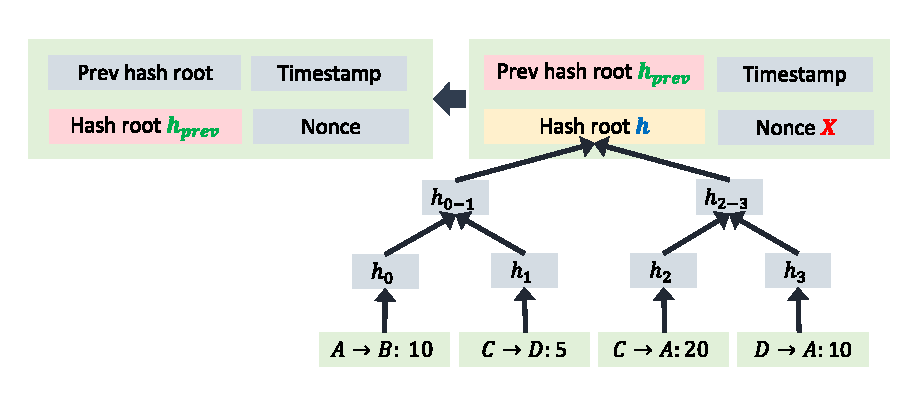
\includegraphics[width=\unitlength,page=1]{Figures/L2_PoW.pdf}}%
  \end{picture}%
\endgroup%
    
\end{minipage}\\
\begin{description}
    \item Given:
        \begin{itemize}
        \item Previous block with hash root $\color{green}h_{\text {prev}}$
        \item Merkle tree consisting of all new transactions with root $\textcolor{blue}h$
        \end{itemize}{}
    \item Find:
        \begin{itemize}
        \item Find a nonce $\texttt{\textcolor{red}{X}}$ such that
        $$
        \operatorname{hash}\left(\textcolor{green}{h_{\text {prev}}}|\textcolor{blue}h|\texttt{\textcolor{red}{X}}\right) \leq \text { difficulty }
        $$
        \end{itemize}{}
\end{description}{}
\paragraph{Properties: }
\begin{itemize}
    \item Difficult to compute
    \begin{itemize}
        \item Current rate in Bitcoin: about 10.2 minutes per block
        \item Probability that a minor succeeds: 10.2 min / fraction of hash power Current hash power: $103,559,611,798 \mathrm{GH} / \mathrm{s}$
    \end{itemize}
    \item Parameterizable cost
    \begin{itemize}
        \item Nodes can adjust the target difficulty
        \item Current difficulty: 15,546,745,765,529
    \end{itemize}{}
    \item Easy to verify
     \begin{itemize}
        \item Other nodes verify that $\operatorname{hash}\left(\textcolor{green}{h_{\text {prev}}}|\textcolor{blue}h|\texttt{\textcolor{red}{X}}\right) \leq \text { difficulty }$

    \end{itemize}{}
    \item Key security assumption
     \begin{itemize}
        \item Attacks infeasible if majority of miners weighted by hash power follow the protocol
    \end{itemize}{}
\end{itemize}{}
\textbf{Note to double spending: } Honest nodes extend the longest valid branch
\paragraph{Incentivizing honest nodes to extend the longest chain}
\begin{itemize}
    \item \textbf{Block reward}. The creator of a block can:
    \begin{itemize}
        \item Include special coin creation transaction in the block 
        \item Choose recipient address of this transaction
        \item Value of transaction is fixed, gets halfed every 210,000 blocks
        \item Block creator ”receives” the reward only if the block ends up on the long-term consensus branch
    \end{itemize}{}
    \item \textbf{Transaction fees}
    \begin{itemize}
        \item Creator of transaction may choose to make output value less than input value. \texttt{\textcolor{blue}{Transaction fee}} = $\sum i n p u t s-\sum o u t p u t s$
    \end{itemize}{}
\end{itemize}{}
\subsection{Bitcoin Scripting:}
\begin{itemize}
    \item \textbf{Data}
    \begin{itemize}
        \item public keys
        \item signatures
    \end{itemize}{}
    \item \textbf{Script opcodes}
    \begin{description}[font=\normalfont,labelwidth=7em,leftmargin =\dimexpr\labelwidth+\labelsep\relax]
        \item [Constants:]  OP\_0, OP\_PUSHDATA\_1, OP\_TRUE
        \item [Flow control:]OP\_IF, OP\_ELSE, ...
        \item [Stack:] OP\_DUP, OP\_SWAP
        \item [Arithmetic:] OP\_ADD, OP\_NEGATE, OP\_LESSTHAN, ...
        \item [Crypto:] OP\_HASH160, OP\_CHECKSIG
        \item [Time:] OP\_CHECKLOCKTIMEVERIFY
    \end{description}{}
    \item \textbf{Important ops and params:}
    \begin{itemize}
        \item Checksig: takes args (\textcolor{orange}{signature}, \textcolor{green}{public key})
    \end{itemize}
\end{itemize}{}
\paragraph{Transaction structure:\newline}
\begin{minipage}{0.5\linewidth}
    \centering      
    \def\svgwidth{\columnwidth}
    %% Creator: Inkscape inkscape 0.92.4, www.inkscape.org
%% PDF/EPS/PS + LaTeX output extension by Johan Engelen, 2010
%% Accompanies image file 'L2_transaction_struct.pdf' (pdf, eps, ps)
%%
%% To include the image in your LaTeX document, write
%%   \input{<filename>.pdf_tex}
%%  instead of
%%   \includegraphics{<filename>.pdf}
%% To scale the image, write
%%   \def\svgwidth{<desired width>}
%%   \input{<filename>.pdf_tex}
%%  instead of
%%   \includegraphics[width=<desired width>]{<filename>.pdf}
%%
%% Images with a different path to the parent latex file can
%% be accessed with the `import' package (which may need to be
%% installed) using
%%   \usepackage{import}
%% in the preamble, and then including the image with
%%   \import{<path to file>}{<filename>.pdf_tex}
%% Alternatively, one can specify
%%   \graphicspath{{<path to file>/}}
%% 
%% For more information, please see info/svg-inkscape on CTAN:
%%   http://tug.ctan.org/tex-archive/info/svg-inkscape
%%
\begingroup%
  \makeatletter%
  \providecommand\color[2][]{%
    \errmessage{(Inkscape) Color is used for the text in Inkscape, but the package 'color.sty' is not loaded}%
    \renewcommand\color[2][]{}%
  }%
  \providecommand\transparent[1]{%
    \errmessage{(Inkscape) Transparency is used (non-zero) for the text in Inkscape, but the package 'transparent.sty' is not loaded}%
    \renewcommand\transparent[1]{}%
  }%
  \providecommand\rotatebox[2]{#2}%
  \newcommand*\fsize{\dimexpr\f@size pt\relax}%
  \newcommand*\lineheight[1]{\fontsize{\fsize}{#1\fsize}\selectfont}%
  \ifx\svgwidth\undefined%
    \setlength{\unitlength}{720bp}%
    \ifx\svgscale\undefined%
      \relax%
    \else%
      \setlength{\unitlength}{\unitlength * \real{\svgscale}}%
    \fi%
  \else%
    \setlength{\unitlength}{\svgwidth}%
  \fi%
  \global\let\svgwidth\undefined%
  \global\let\svgscale\undefined%
  \makeatother%
  \begin{picture}(1,0.57532784)%
    \lineheight{1}%
    \setlength\tabcolsep{0pt}%
    \put(0,0){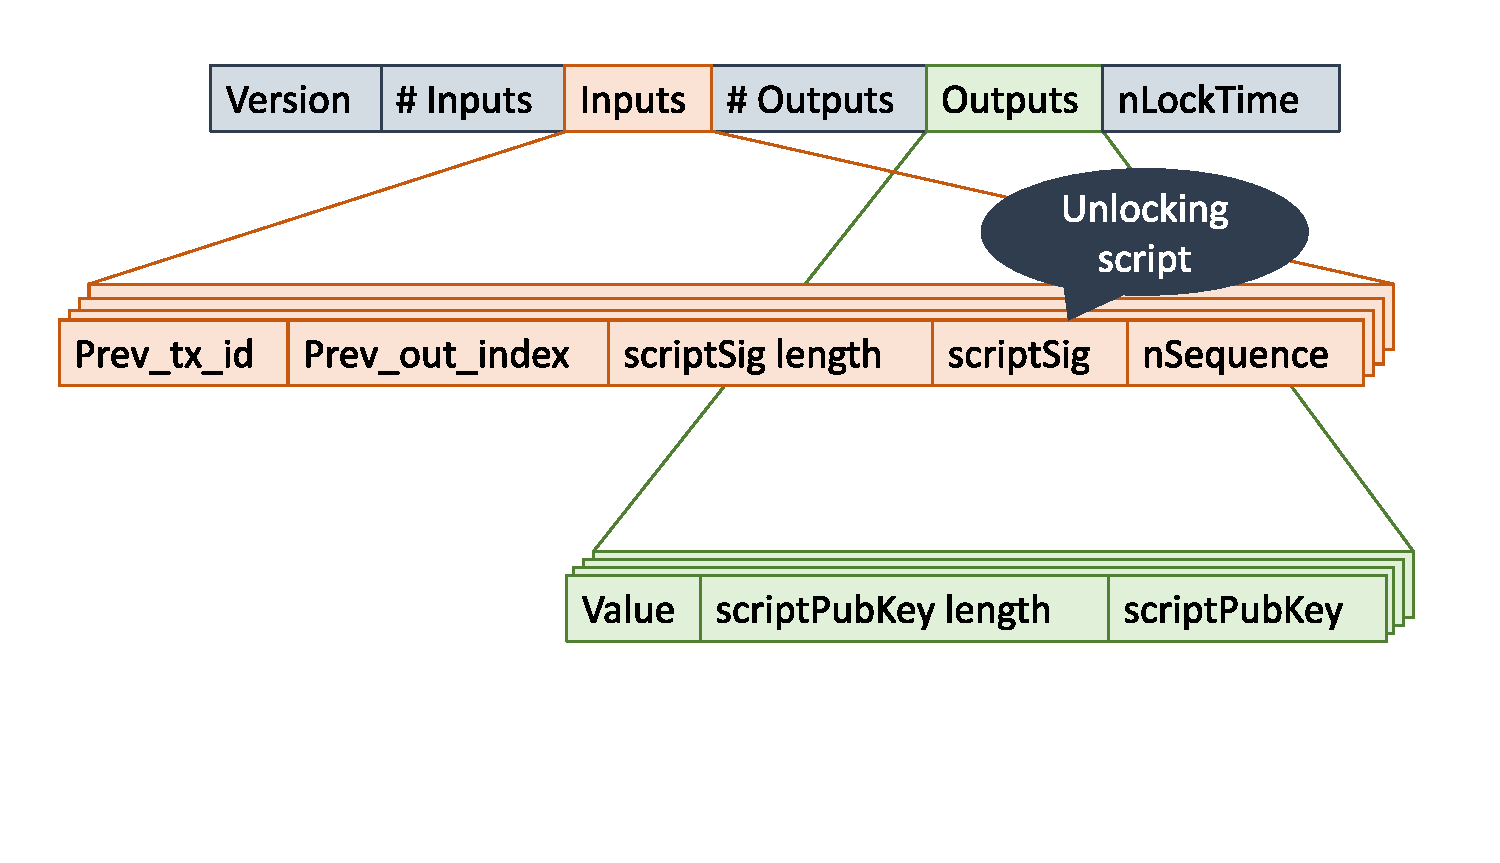
\includegraphics[width=\unitlength,page=1]{Figures/L2_transaction_struct.pdf}}%
  \end{picture}%
\endgroup%
    
\end{minipage}
TODO unlock/locking script\newline
\textbf{Common Bitcoin scripts}\newline
\begin{minipage}{0.5\linewidth}
    \centering      
    \def\svgwidth{\columnwidth}
    %% Creator: Inkscape inkscape 0.92.4, www.inkscape.org
%% PDF/EPS/PS + LaTeX output extension by Johan Engelen, 2010
%% Accompanies image file 'L2_bitcoin_scripts.pdf' (pdf, eps, ps)
%%
%% To include the image in your LaTeX document, write
%%   \input{<filename>.pdf_tex}
%%  instead of
%%   \includegraphics{<filename>.pdf}
%% To scale the image, write
%%   \def\svgwidth{<desired width>}
%%   \input{<filename>.pdf_tex}
%%  instead of
%%   \includegraphics[width=<desired width>]{<filename>.pdf}
%%
%% Images with a different path to the parent latex file can
%% be accessed with the `import' package (which may need to be
%% installed) using
%%   \usepackage{import}
%% in the preamble, and then including the image with
%%   \import{<path to file>}{<filename>.pdf_tex}
%% Alternatively, one can specify
%%   \graphicspath{{<path to file>/}}
%% 
%% For more information, please see info/svg-inkscape on CTAN:
%%   http://tug.ctan.org/tex-archive/info/svg-inkscape
%%
\begingroup%
  \makeatletter%
  \providecommand\color[2][]{%
    \errmessage{(Inkscape) Color is used for the text in Inkscape, but the package 'color.sty' is not loaded}%
    \renewcommand\color[2][]{}%
  }%
  \providecommand\transparent[1]{%
    \errmessage{(Inkscape) Transparency is used (non-zero) for the text in Inkscape, but the package 'transparent.sty' is not loaded}%
    \renewcommand\transparent[1]{}%
  }%
  \providecommand\rotatebox[2]{#2}%
  \newcommand*\fsize{\dimexpr\f@size pt\relax}%
  \newcommand*\lineheight[1]{\fontsize{\fsize}{#1\fsize}\selectfont}%
  \ifx\svgwidth\undefined%
    \setlength{\unitlength}{568.92860232bp}%
    \ifx\svgscale\undefined%
      \relax%
    \else%
      \setlength{\unitlength}{\unitlength * \real{\svgscale}}%
    \fi%
  \else%
    \setlength{\unitlength}{\svgwidth}%
  \fi%
  \global\let\svgwidth\undefined%
  \global\let\svgscale\undefined%
  \makeatother%
  \begin{picture}(1,0.5386064)%
    \lineheight{1}%
    \setlength\tabcolsep{0pt}%
    \put(0,0){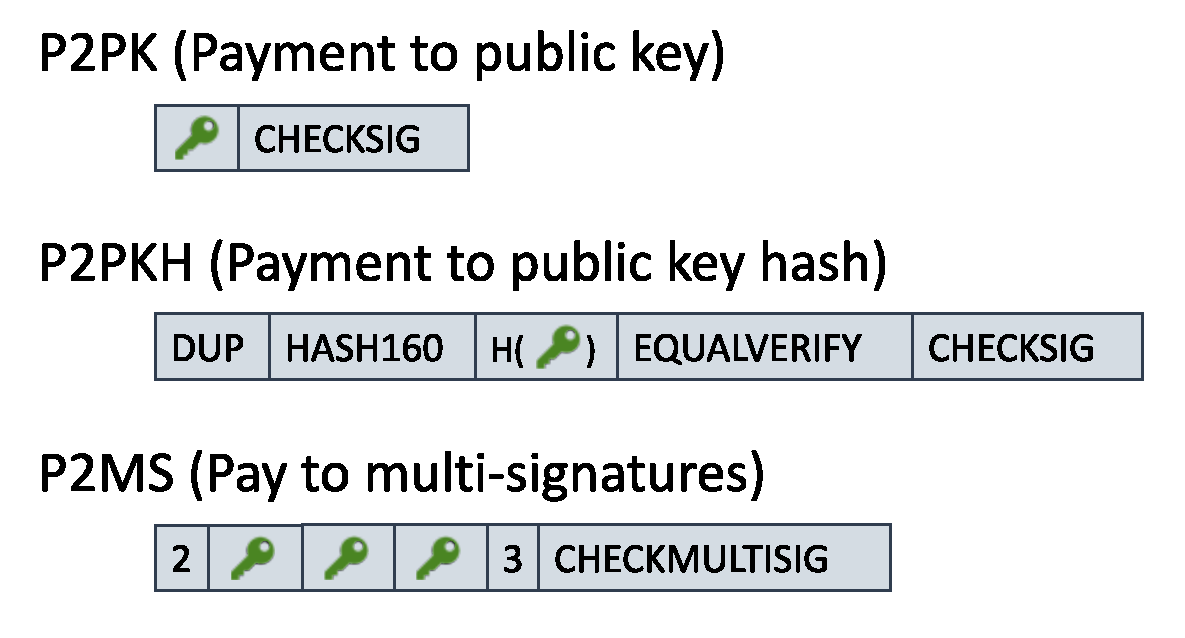
\includegraphics[width=\unitlength,page=1]{Figures/L2_bitcoin_scripts.pdf}}%
  \end{picture}%
\endgroup%
    
\end{minipage}
\paragraph{Bitcoin script Miscellaneous}
\begin{itemize}
    \item BitML: Language for Bitcoin smart contracts
    \item Oracles
    \item Escrow and arbitration
    \item Fair multi-party lotteries
    \item Gambling games (Poker)
    \item Crowdfunding
\end{itemize}{}
\paragraph{Bitcoin scripts Restrictions}
\begin{itemize}
    \item No loops
    \item No signature verification on arbitrary messages
    \item No multiplication and shifting
    \item No arithmetic on long numbers
    \item No concatenation on bitstrings
\end{itemize}
